\section{Reconfiguring \tunnels}\label{s:reconfig}
\begin{listing}[t]
\begin{minted}[linenos, breaklines]{rust}
// Server-side code to "select" a peer-compatible sharding impl. and between DPDK datapaths. 
let ser = SerializeChunnel::new(/*...*/);
let shrd = select!(MboxShard::new(/*..*/), 
        ClientShard::new(/*..*/));
let dp = select!(DpdkThread::new(/*...*/),
    DpdkInline::new(/*...*/));
let handle = dp.handle();
// conns: a stream of incoming connections.
let conns = tbm::make_stack!(ser, shrd, dp).listen(addr);
/* application logic... */
// trigger a re-configuration to the `DpdkInline` chunnel.
handle.reconfigure(DpdkInline);
\end{minted}
\vspace{-10pt}
\caption{\name applications use \texttt{select} in their \tunnel stack to specify options for reconfiguration.}\label{l:select}
\vspace{-10pt}
\end{listing}
\noindent
The uniform interface \tunnels provide enables reconfiguration in \name.
Recall that each \tunnel in \name is associated with a datapath structure that implements the \texttt{ChunnelDatapath} trait. 
A \name connection that uses the \tunnel instantiates an instance of its datapath structure; the \tunnel's connection state is stored in this structure.
Reconfiguring, \ie replacing one \tunnel with another, thus merely requires transferring the connection state from the old \tunnel's datapath structure to the new one and swapping it into the connection structure. 
We detail our reconfiguration API and mechanism below.

\eat{
\begin{outline}
  \1 As we explained before, reconfiguration in \name means changing \tunnel implementations.
  \1  Using \tunnels enables reconfiguration.
    \2 Recall that a \name connection is made of recursively composed \texttt{ChunnelDatapath}s.
    \2 Thus, the state for each \texttt{ChunnelDatapath} in the connection is in a nice little box, and we can plug and unplug other \texttt{ChunnelDatapath}s around it.
    \2 Thus, the strategy for reconfiguration, \ie replacing one \tunnel (say \texttt{AChunnel}) with another  (\texttt{BChunnel}) in a connection, is to first
    check compatibility between the B's implementation and implementations used by other endpoints in the connection, 
    \3 then call the \texttt{BChunnel}'s \texttt{connect\_wrap} function on the \texttt{ChunnelDatapath} that \texttt{AChunnel} previously encapsulated.
    \3 Then, \name needs to help the \texttt{BChunnelDP}\notepanda{A careful reader might be confused about what is a \texttt{BChunnelDP}} translate connection state from A's \tunnel implementation, and finally switch over to the new implementation. 
\end{outline}
}

\subsection{Reconfiguration API} 
Listing~\ref{l:select} shows how an application might implement a function that reconfigures connections.
Developers can express a choice between \tunnels using  \name's \texttt{select} type, shown on lines 3 and 5.
The \texttt{select} type encapsulates both \tunnels and uses one of them (according to a developer-specified preference order) when instantiating a connection.
\texttt{select} can also encapsulate two \tunnel \emph{stacks}, which can in turn contain additional instances of \texttt{select}. When instantiating or reconfiguring a connection, \name considers all stacks in the resulting tree of possibilities.
Once a connection is established, the application can use the returned handle (line 7) to call \texttt{reconfigure} and change this decision.

When implementing the \texttt{reconfigure} function, \name must consider the type of \tunnel being reconfigured. 
While all reconfiguration requires changing the host's \tunnel implementation (we refer to this step as \emph{unilateral} reconfiguration),
reconfiguring some \tunnels additionally requires agreement between all communicating hosts. 
We refer to this step as \emph{multilateral} reconfiguration and reuse \name's negotiation (\S\ref{s:negotiation}) to ensure safety in this case.
The DPDK \tunnel (line 5--6) is an example of a \tunnel that only requires unilateral reconfiguration, while the sharding \tunnel (line 3--4) requires both unilateral and multilateral reconfiguration.
\tunnel implementors indicate whether multilateral reconfiguration is necessary by implementing a \texttt{capabilities()} function (Listing~\ref{l:chunnel} lines 12-13). 

We show an example of reconfiguration in Figure~\ref{f:reconfig}, where we replace one \tunnel, a Kernel UDP socket \tunnel, with a DPDK \tunnel in the connection.
\footnote{\name also supports reconfiguring multiple \tunnels together, amortizing reconfiguration costs.}
First, \name checks compatibility between DPDK's implementation and implementations used by other endpoints in the connection. In this case, the \tunnel is unilateral, so the change is trivially compatible.
Then, \name calls DPDK's \texttt{connect\_wrap} function to initialize it (recall that DPDK's \texttt{connect\_wrap} function bootstraps connections from the unit type). Note that changing this specific \tunnel implementation requires reconfiguring all the connections on the host, since using DPDK often requires exclusive access to the NIC.
This why the lock shown in Figure~\ref{f:reconfig}'s step \raisebox{.5pt}{\textcircled{\raisebox{-.9pt} {1}}} is necessary; we discuss this further in \S\ref{s:impl-reconfig}. 
Then, \name helps the new DPDK connection type translate the connection state from the kernel's \tunnel implementation (\raisebox{.5pt}{\textcircled{\raisebox{-.9pt} {2}}}).
For these \tunnels, the state is simply a list of active connections and the ports they are listening on, but other \tunnels may include other useful state such as sequence numbers.
Finally, \name switches to the new implementation (\raisebox{.5pt}{\textcircled{\raisebox{-.9pt} {3}}}).
  
\begin{figure}
    \centering
    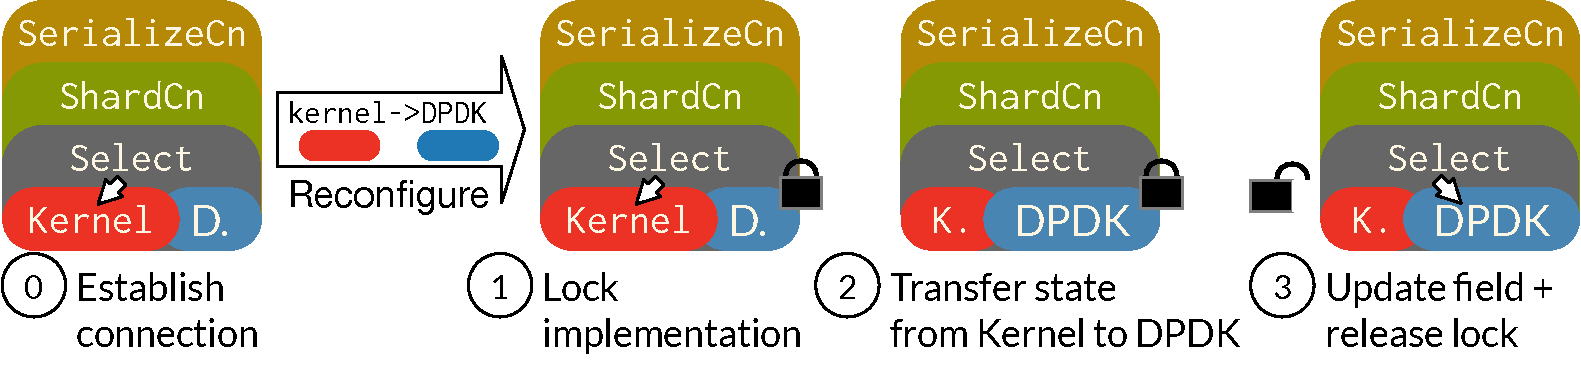
\includegraphics[width=\columnwidth]{img/reconfig-panda-proposal}
    \vspace{2pt}
    \caption{\name reconfigures connections using \texttt{Select}, which can safely change its encapsulated \tunnel implementation.}
    \label{f:reconfig}
\end{figure}
\eat{
\begin{outline}
\0 \paragrapha{Mechanism}
  \1 Listing~\ref{l:select} shows how an application might implement a function that reconfigures connections.
  \1 To express a choice between \tunnels, we provide \name's \texttt{select} type, seen on lines 3 and 5.
  
  \1 The \texttt{select} encapsulates both \tunnels and uses one of them (according to a preference order the developer specifies) when instantiating a connection.
    \2 \texttt{select} can also encapsulate two \tunnel stacks, including those which themselves contain instances of \texttt{select}. When instantiating or reconfiguring a connection, \name considers all stacks in the resulting tree of possibilities.
  
  \1 Later, via a returned handle (line 7), the application can call \texttt{reconfigure} to change this decision.

  
  \1 When implementing this \texttt{reconfigure} function, \name must take into account the type of \tunnels being reconfigured. 
    \2 All reconfiguration requires changing the \tunnel implementation used by the connection, we refer to this step as \emph{unilateral} reconfiguration (\S\ref{s:impl-reconfig}).
        \3 For example, switching between different DPDK datapath structures (shown on lines 5-6) does not depend on what connection peers are doing. 

    \2 In addition, some \tunnels require agreement between all connected peers. Implementors indicate this is necessary by implementing an appropriate \texttt{capabilities()} function (Listing~\ref{l:chunnel} lines 12-13), and if necessary \name also uses its negotiation protocol (\S\ref{}) to perform \emph{multilateral} reconfiguration.
        \3 For example, selecting sharding implementations (lines 3-4) requires agreement on the sharding policy from connection peers. %
  \1 \fixme{check point for flow:} Note that multiple \tunnels can be reconfigured at a time, in which case \name amortizes the cost of each step. 

\0 When re-configuring a multilateral \tunnel, we must ensure that all peers agree on when to switch to a new \tunnel stack. \name uses a two-phase commit to choose a commit point when \tunnel
implementations are switched. If any peer refuses to switch (or times out), reconfiguration fails.\footnote{Because all peers must accept the transition for it to commit, a faulty peer cannot force all connection participants to switch stacks.}
We demonstrate this process in \S\ref{s:eval:pubsub}.

  \1 \fixme{check point for flow:} Note that multiple \tunnels can be reconfigured at a time, in which case \name amortizes the cost of each step. 
\end{outline}
}

\subsection{Reconfiguration Mechanism}\label{s:impl-reconfig}
Here we explain how we switch implementations on a single host.
The core challenge lies in ensuring that \name preserves state as it switches \tunnel implementations. 
Individual \tunnels may have state (\eg the DPDK example from before relies on host-wide NIC configuration), so when re-configuring a connection \name allows the new \tunnel to initialize the corresponding state.
Thus, for safety, we need to ensure that there is a \emph{switch point} after which no connection on any thread uses the old implementation or any of its state.
\name must ensure that the state is copied to the new implementation before this switch point.

We can implement reconfiguration by protecting the encapsulated connection with a lock. The \texttt{reconfigure()} call initializes the newly encapsulated connection, locks the connection state, and updates it to use the newly initialized connection.
In this implementation, the switch point is when \texttt{reconfigure()} releases the connection lock.
We describe a lock-free optimization in  \S\ref{s:impl}.

When re-configuring a multilateral \tunnel, we must ensure that \emph{all} peers agree on the switch point. 
Therefore, the negotiation protocol occurs while \texttt{reconfigure()} holds the connection lock.
\name listens for negotiation protocol packets concurrently with the application. If it receives one, it takes the connection lock (this is the switching point) before sending any negotiation response that could result in a reconfiguration to prevent any race condition between the negotiation response and the subsequent application data packet from the application. 
During reconfiguration, \name uses a two-phase commit to ensure that all endpoints agree on when to switch.
If any peer refuses to switch (or times out), reconfiguration fails.\footnote{Because all peers must accept the transition for it to commit, a faulty peer cannot force other connection participants to switch \tunnel stacks.}
We demonstrate this process in \S\ref{s:app:pubsub}.

\section{Negotiation}\label{s:negotiation}
\name's negotiation protocol ensures compatibility for the \tunnel stacks used by hosts communicating using a connection and is used when connections are established or reconfigured. 
Two \tunnels are \emph{compatible} if data sent by one can be processed by the other.
For example, two serialization \tunnels are compatible if data serialized by one can be deserialized by the other. 
Checking compatibility requires knowledge of the \tunnel stack being used at all endpoints and thus requires communication.
In this section, we first describe our negotiation protocol for connections that have two endpoints, \ie point-to-point connections.
Then, in \S\ref{s:multiparty}, we describe a more general protocol that supports connections with more than two endpoints. 
The larger number of endpoints brings additional challenges and complexity, and hence, we use both protocols, choosing between them depending on the type of connection.

\subsection{Negotiation Protocol}\label{s:neg-proto}
To begin negotiation, \name needs a channel over which it can communicate with its peer.
Therefore, we require that the bottom layer of the \tunnel stack always be able to establish a compatible initial connection (by transforming the unit type \texttt{()}). 
We refer to this initial connection as \emph{base connection}, and only require that it provide best-effort delivery.
\name implements a simple reliability and ordering protocol that it uses for negotiation.
Using the base connection, the client sends the server a message describing its \tunnel stack (represented as a set of \tunnel options). 
On receiving this message, the server checks whether its connection has a \tunnel stack (making a choice for each instance of \texttt{select}) that is compatible with the client's options (\S\ref{s:check-compat}). If it finds a compatible stack, it sends it to the client; otherwise, it returns an error to the client and terminates the connection.
Both the server and the client then use recursive \texttt{connect\_wrap} calls (\S\ref{s:chunnel}) to initialize the selected stack.

Each \name connection is associated with a single address, which is used during negotiation.
Therefore, \name does not support connection-less sockets.
This restriction also holds for multi-party connections (\S\ref{s:multiparty}), where the address might represent a pub/sub topic or a multicast IP address.
In cases where a \tunnel, \eg a sharding \tunnel, can send data to multiple endpoints, we require either multi-party negotiation (\S\ref{s:multiparty}) or that all endpoints support the same set of \tunnel implementations.
This ensures that negotiating with one endpoint is sufficient to ensure compatibility with the rest.
Thus, after negotiation, \name returns a nonce that encodes which \texttt{select} branches to use;
a \tunnel can use this nonce to inform endpoints about the stack they should use with the given client.
We adopted this approach for the load-balancing \tunnel in \S\ref{s:app:lb}.



\subsection{Checking Compatibility}\label{s:check-compat}
The negotiation protocol requires \name to check compatibility between pairs of \tunnels. 
A tempting approach to do so would be to use static analysis to check compatibility between \tunnel implementations. However, \name does not constrain how developers write \tunnels, and checking compatibility is at least as hard as checking equivalence, and well-known results in logic show that checking equivalence between programs is undecidable~\cite{sipser13}. 
Therefore, in \name, we adopt a simpler approach where \tunnels provide runtime type information
that \name uses to check compatibility.
However, we allow for a more general version of compatibility and allow \tunnels with different types to be compatible.
To allow for this, \name requires developers to provide capabilities (opaque to \name) that implement a comparison function for checking compatibility between \tunnels (Listing~\ref{l:chunnel} lines 12-13). 

\tunnel developers can either define a new capability type (or reuse an existing one to indicate compatibility with that \tunnel), and return an instance of this type when \name calls the \tunnel's \texttt{capability} function. 
A capability type needs to implement the \texttt{Capability} interface, which requires defining a comparison function, and must be serializable. We do not assume that capabilities are standardized; instead, we only require that developers writing networked programs that communicate with each other (\eg a client and a server) use the same capability types.
Thus, capabilities allow \tunnel developers to indicate \emph{relative} compatibility between different implementations.
For example, if the ProtoBuf developers provide a software reference implementation of their serialization library, a later compatible implementation based on ProtoACC~\cite{protoacc} can reuse the same capability types to indicate compatibility, as can any future implementations.

In practice, we found that we can encode \tunnel capabilities as a set of labels and that checking compatibility between them requires either checking that the sets are equal -- we refer to this as ``exact-match'' -- or that there is a non-empty intersection between sets -- we refer to this as ``composition''.
So, to check \tunnel stack compatibility, \name ensures that ``exact-match'' capabilities (such as serialization) are present in both compared stacks, and that ``compositional'' capabilities (such as sharding) are present in at least one.
If there are multiple possibilities, \name uses the developer's specified preference order (\ie the branch listed first).

\subsection{Multi-Party Negotiation}\label{s:multiparty}
\name supports connections with an arbitrarily large number of endpoints communicating over a single connection (\eg multicast or publish-subscribe). 
Before designing a negotiation protocol for this scenario,  we need to first determine how negotiation works in a multi-endpoint setting. 
A point-to-point connection only exists for as long as the client and server are communicating and does not need to consider cases where endpoints join after the negotiation step has finished,
but with multiple endpoints
we can neither assume that all endpoints are known when a connection is first established nor can we require that all endpoints connect at the same time. 
As a result, multi-party negotiation must allow (a) endpoints to recover a connection's datapath stack even if they did not participate in its negotiation, and (b) when necessary, allow endpoints to trigger another round of negotiation to transition to a different datapath stack. 

We implement a ``rendezvous-based'' negotiation protocol for the multi-endpoint case. We implement negotiation using a key-value store that can be accessed by all endpoints. The key-value store is also responsible for recording the negotiated datapath stack, thus allowing endpoints to recover the connection's datapath stack even when they do not participate in the negotiation. We require that the key-value store support serializable multi-key transactions. However, we do not impose other requirements, and we allow the use of either single-node key-value stores (\eg Redis) or replicated consensus-based stores (\eg etcd). 
While a failure of this key-value store would prevent new endpoints from joining a multi-endpoint connection, it would not impact endpoints that have already joined. 
Furthermore, the negotiation state is not shared across connections, and thus the key-value store can be easily sharded for scalability. While using an external-key value store makes establishing a multi-endpoint connection take longer, any algorithm for multi-endpoint negotiation requires agreement and would thus impose similar performance costs.

A peer starts multi-party negotiation by connecting to the key-value store and proposing a \tunnel implementation stack, using compare-and-swap (\eg via a transaction) to check for an existing stack.
If the compare-and-swap operation succeeds, the peer can safely use the \tunnel implementation stack it proposed. 
Otherwise, the key-value store returns the \tunnel implementation stack already in place amongst the existing connection participants along with the number of participants in the connection.
The new peer then uses the same stack comparison procedure described in \S\ref{s:check-compat} to determine its local stack's compatibility.
The peer can then use this stack to create its connection or propose a reconfiguration as per \S\ref{s:impl-reconfig}.
